\documentclass[9pt,twocolumn,twoside]{pnas-new}
% Use the lineno option to display guide line numbers if required.
\usepackage{subcaption}
\templatetype{pnasresearcharticle} % Choose template 

%\title{Invariances in gain control of olfactory receptor neurons enhances the combinatorial coding fidelity}
%\title{Invariances in gain control of olfactory receptor neurons enhances the fidelity of an odor code}
%\title{Universal front-end gain control aids robust combinatorial odor coding in naturalistic environments}
%\title{Weber-Fechner gain control in olfactory receptor neurons enhances combinatorial coding fidelity}
%\title{Weber-Fechner gain control in olfactory receptor neurons enhances the fidelity of odor coding}
%\title{Weber-Fechner gain control enhances the fidelity of combinatorial odor coding}
\title{Front-end Weber-Fechner gain control enhances the fidelity of combinatorial odor coding}


% Use letters for affiliations, numbers to show equal authorship (if applicable) and to indicate the corresponding author
\author[a]{Nirag Kadakia}
\author[a,b]{Thierry Emonet} 

\affil[a]{Department of Molecular, Cellular, and Developmental Biology}
\affil[b]{Department of Physics, Yale University, New Haven, CT 06511}

% Please give the surname of the lead author for the running footer
\leadauthor{Kadakia} 

% Please add here a significance statement to explain the relevance of your work
\significancestatement{In insect olfaction, odors are believed to be encoded by the distinct spatiotemporal patterns of activity they elicit in sensing neurons. Here, we investigate how these patterns would be maintained in naturalistic environments, where odor concentrations can vary rapidly, and where ethologically-relevant odors often mix with backgrounds. We show that a robust mechanism of response adaptation, the Weber-Fechner Law of perceived difference, which was recently observed in \textit{Drosophila}, may play a vital role in maintaining these odor codes. While the Weber-Fechner Law is known to maintain sensitivity in single-channel systems, here we illustrate its general applicability to multi-channel systems in which responses may be broad and highly overlapping.}

% Please include corresponding author, author contribution and author declaration information
\authorcontributions{N.K. and T.E. conceived the project, analyzed the results, and wrote the manuscript. N.K. performed all calculations. T.E. supervised the project.}
\authordeclaration{Authors declare no conflict of interest}
%\equalauthors{\textsuperscript{1}A.O.(Author One) and A.T. (Author Two) contributed equally to this work (remove if not applicable).}
\correspondingauthor{\textsuperscript{2}To whom correspondence should be addressed. E-mail: thierry.emonet@yale.edu}

% Keywords are not mandatory, but authors are strongly encouraged to provide them. If provided, please include two to five keywords, separated by the pipe symbol, e.g:
\keywords{Odor coding $|$ Sensory systems $|$ Weber's Law $|$ Olfactory receptor neurons $|$ \textit{Drosophila melanogaster}} 

\begin{abstract}
    Odor identity is encoded by spatiotemporal patterns of activity in olfactory receptor neurons (ORNs). In natural environments, the intensity and timescales of odor signals can span several orders of magnitude, and odors can mix with one another, potentially scrambling the combinatorial code mapping neural activity to odor identity. Recently, it was demonstrated that for many distinct odorants, individual ORNs scale their gain inversely with mean odor concentration according to the Weber-Fechner Law of psychophysics. Here we  use a minimal biophysical model of signal transduction, ORN firing, and signal decoding to investigate the implications of this front-end scaling law for the neural representations of odor identity. 
    %We find that a recently-characterized adaptive scaling law in the \textit{Drosophila} olfactory periphery may help preserve neural representations of odor identity, despite these possible confounds. ORN gain scales inversely with concentration according to the Weber-Fechner law of psychophyics
    %odor- and receptor-independent adaptive scaling law in the \textit{Drosophila} olfactory periphery -- ORN gain scales inversely with odor concentration according to the Weber-Fechner law of psychophysics -- may. 
    We find that Weber-Fechner scaling enhances coding capacity and promotes the reconstruction of odor identity from dynamic odor signals, even in the presence of confounding background odors and rapid intensity fluctuations. We show that these enhancements are further aided by downstream transformations %of neural signals %, such as normalization and divergence 
    in the antennal lobe and mushroom body. Thus, despite the broad overlap between individual ORN tuning curves, a mechanism of front-end adaptation, when endowed with Weber-Fechner scaling, may play a vital role in preserving representations of odor identity in naturalistic odor landscapes.
    
    %a parsimonious, dynamic adaptive mechanism at the front-end of the olfactory circuit may play a central role in preserving representations of odor identity in naturalistic odor landscapes.
    
    %Further, front-end adaptation acts in concert with downstream mechanisms, such as normalization and divergence in the \textit{Drosphila} antennal lobe and mushroom body, reveals that front-end adaptation, besides its known role in enhancing detection of temporal variations in signal intensity, also contributes significantly to coding and decoding of odor identity.  
    %Thus, despite the broad overlap of ORN tuning curves, a mechanism of front-end adaptation, when endowed with Weber-Fechner scaling, may play a vital role in preserving representations of odor identity in naturalistic odor landscapes.
\end{abstract}

\dates{This manuscript was compiled on \today}
\doi{\url{www.pnas.org/cgi/doi/10.1073/pnas.XXXXXXXXXX}}

% Added to get write linespread as published articles
\linespread{0.9}

% Set paragraph spacing to zero.
\setlength{\parskip}{0cm plus0mm minus0mm}

\begin{document}


% Optional adjustment to line up main text (after abstract) of first page with line numbers, when using both lineno and twocolumn options.
% You should only change this length when you've finalised the article contents.
%\verticaladjustment{-2pt}

\maketitle
\thispagestyle{firststyle}
\ifthenelse{\boolean{shortarticle}}{\ifthenelse{\boolean{singlecolumn}}{\abscontentformatted}{\abscontent}}{}

%%%%%%%%%%%%%%%%%%%%%%%%%%%%%%%%%%%%%%%%%%%%%%%%%%%%%%%%%%%%%%%%%
%%%%%%%%%%%%    		INTRODUCTION	    		%%%%%%%%%%%%%
%%%%%%%%%%%%%%%%%%%%%%%%%%%%%%%%%%%%%%%%%%%%%%%%%%%%%%%%%%%%%%%%%




Animals identify and discriminate odors using olfactory receptors (Ors) expressed in olfactory receptor neurons (ORNs)~\cite{chemoreceptors_review,buck1991novel,or_discovery_carlson,or_discovery_vosshall}. Individual ORNs, which typically express a single Or, respond to many odorants, while individual odorants activate many distinct ORNs~\cite{friedrich1997combinatorial,hallem_carlson,mosquito_combinatorial_coding,nara2011large}. Odors are  thus encoded by the combinatorial patterns of activity they elicit in the sensing periphery~\cite{malnic1999combinatorial, mosquito_combinatorial_coding, hildebrand1997mechanisms, hallem_carlson, debryune_odor_coding, friedrich1997combinatorial}, patterns  decoded downstream into behavioral response~\cite{early_olfactory_processing}.  Still, ethologically-relevant odors are often mixed with background ones~\cite{odor_backgrounds} and intensity can vary widely and rapidly as odors are carried by the wind~\cite{murlis_odor_plumes, fluid_dynamics_chemosensory, celani, carde_navigation}. How are odors recognized reliably despite these confounds? %Various mechanisms have been suggested. 
In \textit{Drosophila melanogaster}, ORN dose response curves exhibit similar Hill coefficients but distinct power-law distributed activation thresholds~\cite{hallem_carlson, si2017invariances}, which together with inhibitory odorants enhance coding capacity~\cite{si2017invariances, Cao_Tu_WL, hallem_carlson, stevens}. In antennal lobe (AL) glomeruli, mutual lateral inhibition normalizes population response, reducing the dependency of activity patterns on odor concentration~\cite{lateral_inh_asahina, divisive_normalization}. Further downstream, sparse connectivity to the mushroom body (MB) helps maintain neural representations of odors, and facilitates compressed sensing decoding schemes~\cite{abbott_axel, litwinkumar, vijay_1}. Finally, temporal features of neural responses contribute to concentration-invariant representations of odor identity~\cite{stopfer_nat_neuro, stopfer_temporal_model, stopfer_temporal_channel, primacy_coding}.

Here we examine how short-time ORN adaptation at the very front-end of the insect olfactory circuit contributes to the fidelity of odor encoding. Our theoretical study is motivated by the recent discovery of invariances in the response dynamics of ORNs expressing the co-receptor Orco. %While for some odor-Or combinations, ORN responses can exhibit large differences, such as super-sustained responses~\cite{montague2011similar} or specialized responses to danger signals~\cite{geosmin}, for many odor-Or combinations the deconvolution of stimulus dynamics from neuron responses produces highly stereotyped filters~\cite{martelli,si2017invariances}. 
The responses of ORNs to diverse odorants presented at the same concentration differ widely due to differences in odor-receptor affinities \cite{hallem_carlson,montague2011similar,geosmin}, and stimulus dynamics (\cite{martelli}. However, downstream from this input nonlinearity, signal transduction and adaptation dynamics that lead to ORN firing exhibit a surprising degree of invariance with respect to odor-receptor identity. Indeed, reverse-correlation analysis of ORN response to fluctuating stimuli produces highly stereotyped, concentration-invariant response filters~\cite{martelli,si2017invariances}, enabling ORNs to maintain response time independent of odor intensity~\cite{martelli, srinivas_elife}.

These properties stem in part from an apparently invariant adaptive scaling law in ORNs: gain varies inversely with mean odor concentration according to the Weber-Fechner Law of psychophysics~\cite{weber1996eh,fechner2012elemente}, irrespective of the odor-receptor combination~\cite{srinivas_elife,cafaro_WL,cao_WL}. The invariance of this relatively fast adaptation ($\sim$250 ms) can be traced back to  feedback mechanisms in odor transduction, upstream of ORN firing~\cite{nagel_wilson_biophysical,cao_WL,cafaro_WL,srinivas_elife}, which depend on the activity of the signaling pathway rather than on the identity of its receptor~\cite{nagel_wilson_biophysical}. 
The generality of the adaptive scaling suggests it could be mediated by the highly conserved Orco co-receptor~\cite{orco_structure,getahun2013insect,getahun2016intracellular,Guo_Smith}. Indeed, phosphorylation sites have been recently identified on Orco, some being implicated in odor desensitization, albeit over much longer timescales~\cite{Guo_Smith_review,Guo_Smith}. 


\begin{figure*}[!tb]
	\centering
	\begin{subfigure}[t]{\linewidth}
		\phantomsubcaption
		\label{fig:tuning_curves_a}
	\end{subfigure}
	\begin{subfigure}[t]{0\linewidth}
		\phantomsubcaption
		\label{fig:tuning_curves_b}
	\end{subfigure}
	\begin{subfigure}[t]{0\linewidth}
		\phantomsubcaption
		\label{fig:tuning_curves_c}
	\end{subfigure}
	\begin{subfigure}[t]{0\linewidth}
		\phantomsubcaption
		\label{fig:tuning_curves_d}
	\end{subfigure}
	\begin{subfigure}[t]{0\linewidth}
		\phantomsubcaption
		\label{fig:tuning_curves_e}
	\end{subfigure}
	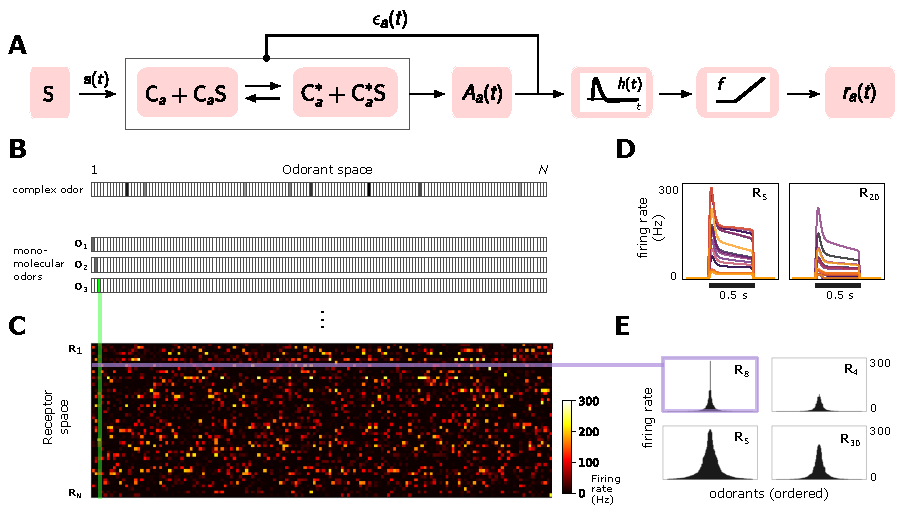
\includegraphics[width=\linewidth]{figures/1_tuning_curves}
	\caption{\footnotesize{
		\textbf{A}~Simple ORN model. Or/Orco complexes $\textup{C}_a$ bind odorant molecules of type $i$ and concentration $s_i$ comprising stimuli $\textup{S}$. Or/Orco complexes stochastically switch between inactive and active states, where the steady-state active fraction is determined by the free energy difference between active and inactive conformation, which in turns depends on odor binding and contribution $\epsilon_a(t)$ from adaptation. We assume the activity feeds back on to the free energy difference of the complexes with timescale $\tau$ to pull the activity to a baseline level $A_{a0}$. ORN firing rates $r_a(t)$ are generated by passing $A_a(t)$ through a linear temporal filter $h(t)$ and a nonlinear thresholding function $f$. 
		\textbf{B}~Odor mixtures are represented by $N$-dimensional vectors $\mathbf s$, whose components $s_i$ are the concentrations of  the individual molecular constituents  of $\mathbf s$. 
		%\textbf{C}~Active binding constants are distributed as a power-law with coefficient $\alpha=0.35$~\cite{si2017invariances}.
		\textbf{C}~The steady state firing response of 50 ORNs to the 150-possible monomolecular odors $\mathbf s = s_i$, given  power-law distributed $K^*_{ai}$~\cite{si2017invariances}.
		\textbf{D}~Temporal responses of two representative ORNs to a pulse stimulus, for several monomolecular odorants (colors); absolute firing rate (top row) and normalized rates (bottom row).
		\textbf{E}~Representative ORN tuning curves (a single row of the response matrix in C, ordered by magnitude). Tuning curves are diverse, mimicking measured responses~\cite{hallem_carlson}.
		}}
		\label{fig:tuning_curves}
\end{figure*}

While in a simple system such as \textit{E. coli} chemotaxis, adaptive feedback via the Weber-Fechner Law robustly maintains sensitivity over concentration changes~\cite{robustness_alon,EmonetReview}, the implication for a multiple-channel system -- which combines information from hundreds of cells with overlapping receptive fields  -- is less straightforward. Here we combine a biophysical model of ORN adaptive response and neural firing with various sparse signal decoding frameworks to explore how ORN adaptation with Weber-Fechner scaling affects combinatorial coding and decoding of odor signals spanning varying degrees of intensity, molecular complexity, and temporal structure. We find that this front-end adaptive mechanism promotes the accurate discrimination of odor signals from backgrounds of varying molecular complexity, and aids other known mechanisms of neural processing in the olfactory circuit to maintain representations of odor identity across environmental changes. %both in static odor environments  and in fluctuating ones.
%We also investigate our framework in the context of the primacy coding hypothesis  -- that odors are encoded entirely by the few earliest responding ORNs~\cite{primacy_coding, primacy_math}, finding that primacy coding is both consistent with and enhanced by front-end adaptation. 


\section*{Results}



%%%%%%%%%%%%%%%%%%%%%%%%%%%%%%%%%%%%%%%%%%%%%%%%%%%%%%%%%%%%%%%%%
%%%%%%%%%%%%    		MODEL DESCRIPTION    		%%%%%%%%%%%%%
%%%%%%%%%%%%%%%%%%%%%%%%%%%%%%%%%%%%%%%%%%%%%%%%%%%%%%%%%%%%%%%%%



\subsection*{Model of ORN sensing repertoire}

We consider a repertoire of $M=50$ Orco-expressing ORN types modeled using a simple extension of a minimal model of odor-to-ORN firing~\cite{srinivas_elife} that reproduces the type of Weber-Fechner adaptation and firing rate dynamics measured in individual \textit{Drosophila} ORNs in response to Gaussian and naturalistic signals. Within ORNs of type $a=1,...,M$, we model Or-Orco complexes as non-selective cation channels~\cite{orco_structure} (Fig.~\ref{fig:tuning_curves_a}) that stochastically switch between active and inactive states, while simultaneously binding to odorants $i$ with dissociation constants, $K^*_{ai}$ and $K_{ai}$, respectively~\cite{nagel_wilson_biophysical,srinivas_elife}. Assuming these processes are faster than other reactions in the signaling pathway, the quasi-steady state active fraction $A_a$ of channels in ORNs of type $a$ reads:
\begin{align}
A_a(t) = \left(1 + e^{\epsilon_a(t)}\frac{1 + \sum_i^N s_i(t)/K_{ai}}{1 + \sum_i^N s_i(t)/K^*_{ai}}\right)^{-1}.
\label{eq:steady_state_act_OR}
\end{align}
$s_i(t)$ are the time-dependent concentrations of the individual monomolecular components of the odor signal $\bf{s}(t)$ at time $t$, and $N=150$ is the size of the molecular odorant space (Fig.~\ref{fig:tuning_curves_b}). Inward currents elicited by activating Or-Orco channels~\cite{orco_structure} eventually result in a negative feedback onto $A_a(t)$~\cite{nagel_wilson_biophysical,srinivas_elife,cao_WL}:
\begin{align}
\tau\frac{d\epsilon_a(t)}{dt} = {A}_{0} - A_a(t).
\label{eq:adaptation_dynamics}
\end{align}
Here, $\tau$ is the adaptation time and $\epsilon_a(t)$ is the free energy difference change due to modifications of the Or-Orco complexes by the short-term adaptation mechanism, which we assume is limited to a finite range $\epsilon_{\textup{L}, a} < \epsilon_a(t) < \epsilon_{\textup{H}, a}$~\cite{srinivas_elife}. Firing rate is minimally modeled by filtering the activity $A_a(t)$ with the double exponential filter $h(t)$ and rectifying nonlinearity $f$~\cite{srinivas_elife}:
\begin{align}
r_a(t)=f\left(h\otimes A_a(t)\right),
\label{eq:firing_machinery}
\end{align}
where $\otimes$ is convolution. When deconvolved from stimulus dynamics, the shapes of the temporal kernels of \textit{Drosophila} ORNs that express Orco are largely receptor- and odor-independent~\cite{martelli,srinivas_elife,si2017invariances}. Moreover, adaptation is not intrinsic to the receptor~\cite{nagel_wilson_biophysical}. Accordingly, $\tau$, $h(t)$ and $f$ are assumed independent of receptor and odorant identities (Note, however, relaxing these invariances does not affect our results; SI text).

We assume that the lower cutoffs $\epsilon_{\textup{L}, a}$ are receptor-dependent and choose them from a normal distribution. This variability ensures that ORNs are activated above quiescence (set at 5 Hz) at distinct stimulus levels~\cite{srinivas_elife, martelli}. Diversity among odor-ORN responses arises mainly from the distribution of chemical dissociation constants (Fig.~\ref{fig:tuning_curves_c}). For simplicity we only consider agonists, i.e. $K^*_{ai}>K_{ai}$, and assume receptors can only bind one odorant at a time. The analysis can easily be extended to include inhibitory odorants, which increases coding capacity~\cite{Cao_Tu_WL}. We choose the dissociation constants from a power law distribution ($\alpha = 0.35$) recently found across ORN-odor pairs in \textit{Drosophila} larvae~\cite{si2017invariances}. For a handful of ORNs we choose a very small value for one of the $K^*_{ai}$ to mimic high responders to private odorants relevant to innate responses. These private odors do not affect the general findings. 
 
While this phenomenological model could be extended to include further details -- e.g. we could relax the quasi-steady-state assumption in Eq.~\ref{eq:steady_state_act_OR} and use a more complex model for neural firing~\cite{srinivas_elife} -- this minimally-parameterized form captures the key dynamical properties of Orco-expressing ORNs relevant to our study: receptor-independent adaptation~\cite{nagel_wilson_biophysical} with Weber-Fechner scaling~\cite{srinivas_elife,cafaro_WL,cao_WL} that maintains response time independent of mean stimulus intensity~\cite{martelli,srinivas_elife}, along with a diversity of both steady state and temporal firing patterns in response to a panel of monomolecular odorants~\cite{hallem_carlson,montague2011similar,stopfer_nat_neuro,stopfer_temporal_channel,stopfer_temporal_model} (Fig.~\ref{fig:tuning_curves_d}-\ref{fig:tuning_curves_e}). 




%%%%%%%%%%%%%%%%%%%%%%%%%%%%%%%%%%%%%%%%%%%%%%%%%%%%%%%%%%%%%%%%%
%%%%%%%%%%%%		CODING CAPACITY SECTION			%%%%%%%%%%%%%
%%%%%%%%%%%%%%%%%%%%%%%%%%%%%%%%%%%%%%%%%%%%%%%%%%%%%%%%%%%%%%%%%




\subsection*{Concentration-invariant preservation of coding capacity and abstract representations of odor identity}

\begin{figure}[!tb]
	\centering
	\begin{subfigure}[t]{\linewidth}
		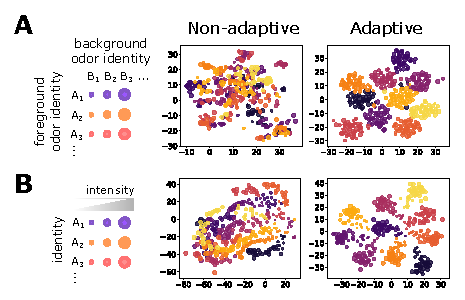
\includegraphics[width=\textwidth]{figures/2_coding_representation}
		\phantomsubcaption
		\label{fig:coding_a}
	\end{subfigure}
	\begin{subfigure}[t]{0\linewidth}
		\phantomsubcaption
		\label{fig:coding_b}
	\end{subfigure}
	\caption{\footnotesize{Front-end adaptation maintains representations of odor identity across background and intensity confounds.
	\textbf{A}~Abstract representation of ORN responses in a low-dimensional embedding. Each point represents the repertoire of ORN firing rates, in response to an odor environment with both a foreground (point color) and background (point size) odor. In the adaptive system, $\epsilon_a$ are set to their steady state values given odor B alone.
    \textbf{B}~Similar to A, but now for odors whose concentrations span 4 decades (represented by point size). Here, the background odor identity is the same for all concentrations. }}
	\label{fig:coding}
\end{figure}


To investigate how front-end Weber-Law adaptation might preserve representations of odor identity within the repertoire of ORN response, we project the 50-dimensional  firing rates $\mathbf r$ down to a 2-dimensional space using t-distributed stochastic neighbor embedding (t-SNE)~\cite{tsne}. We first perform this embedding for an adaptive or non-adaptive system interacting with an odor environment containing a foreground odor A atop a background odor B (Fig.~\ref{fig:coding_a}). Both odors are sparse mixtures, with $K < N$ odorants of similar concentrations, odor "identity" being the particular set of odorants in the mixture. Adaptation to the background is enacted by setting $\epsilon_a$ to their steady state values (via Eq.~\ref{eq:adaptation_dynamics}) in response to odor B alone. With adaptation in place, responses cluster by the identity of odor A, suggesting that ORN responses appropriately encode the identity of novel odors irrespective of background signals -- once these backgrounds have been ``adapted away'' (Fig.~\ref{fig:coding_a}). This is notable, since, due to the combinatorics of ORN response (Fig.~\ref{fig:tuning_curves_c}), the adapted $\epsilon_a$ distributions are themselves heavily dependent on background identity. Responses in the non-adaptive system, meanwhile, exhibit no such clustering (Fig.~\ref{fig:coding_a}).
A similar separation by odor identity is preserved in the adaptive system if we consider responses across different intensities (Fig.~\ref{fig:coding_b}). 

Preservation of these representations is enabled by the preservation of coding capacity. Accordingly, we calculated the mutual information between odor and ORN response in time, verifying that the the adaptive system retains coding capacity as it confronts novel odors (Fig.~S1). The non-adaptive system maintains coding capacity, though in a far more limited range of odor concentration.

%The loss of coding capacity in the non-adaptive system, together with the confounding of abstract representations of odor identity suggests that universal front-end adaptative feedback helps preserves odor identitity within the ensemble of ORN response.


%To investigate how front-end adaptation affects coding capacity, we calculate the mutual information (MI) between odor signal $\mathbf s=\mathbf s_A +\mathbf s_B$ and response $\mathbf r$ as a function of signal intensity, with and without adaptation. A step of odor A, $\textbf{s}_A$,  is followed by a step of odor B at some later time much longer than the ORN adaptation timescale $\tau$. 
%turns on at time~$t_A$ and a step of odor B, $\mathbf s_B$ turns on at some later time~$t_B$ (Fig.~\ref{fig:coding_a}). Both odors have similar intensities. 
%In the non-adaptive case, MI peaks around the region of maximum sensitivity ($\sim 10^2$ a.u.) after $t_A$ (Fig.~\ref{fig:??}). The adaptive system mimics the non-adaptive system at $t_A$,  before adaptation has kicked in (Fig.~\ref{fig:coding_c}). In time, adaptation causes the sensitivity to decrease, and the mutual information peak shifts to higher concentrations. Eventually, all ORNS are firing at adapted baseline and mutual information is mostly eliminated. However, having now adjusted its regime of maximum sensitivity to the presence of odor A, the system can respond appropriately to odor B: the MI at $t_B$ is nearly 6 bits across 3 decades of concentration.

%%%%%%%%%%%%%%%%%%%%%%%%%%%%%%%%%%%%%%%%%%%%%%%%%%%%%%%%%%%%%%%%%
%%%%%%%%%%%%    		SIGNAL DECODING      	     %%%%%%%%%%%%
%%%%%%%%%%%%%%%%%%%%%%%%%%%%%%%%%%%%%%%%%%%%%%%%%%%%%%%%%%%%%%%%%




\begin{figure*}[t]
	\centering
	\begin{subfigure}[t]{17.7cm}
		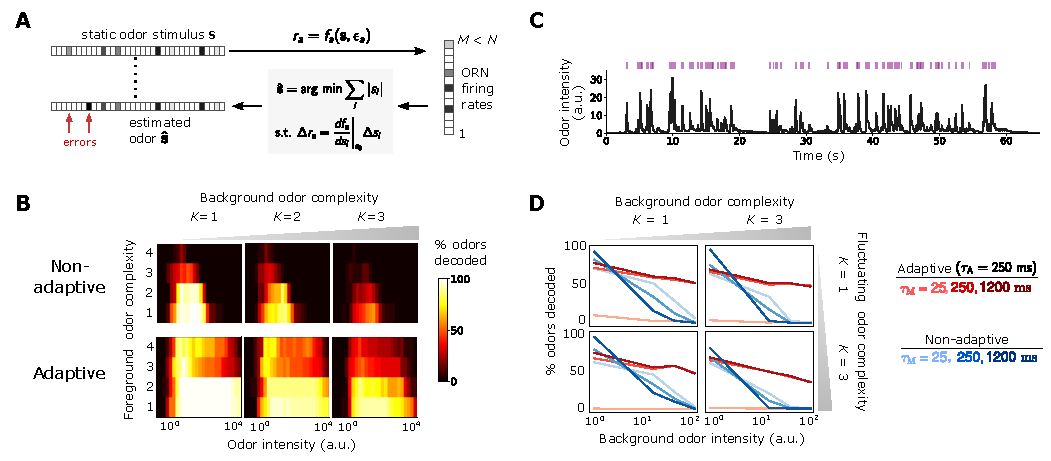
\includegraphics[width=17.7cm]{figures/3_decoding_temporal}
		\phantomsubcaption
		\label{fig:decoding_a}
	\end{subfigure}
	\begin{subfigure}[t]{0\linewidth}
		\phantomsubcaption
		\label{fig:decoding_b}
	\end{subfigure}
	\begin{subfigure}[t]{0\linewidth}
		\phantomsubcaption
		\label{fig:decoding_c}
	\end{subfigure}
	\begin{subfigure}[t]{0\linewidth}
		\phantomsubcaption
		\label{fig:decoding_d}
	\end{subfigure}
	\begin{subfigure}[t]{0\linewidth}
		\phantomsubcaption
		\label{fig:decoding_e}
	\end{subfigure}
	\caption{\footnotesize{Front-end adaptation promotes accurate odor decoding in static and naturalistic odor environments.
    \textbf{A}~Odor stimuli produce ORN responses via odor-binding and activation and firing machinery, as described by Eqs.~\ref{eq:steady_state_act_OR}-\ref{eq:firing_machinery}. Odors are then decoded using compressed sensing by linearizing around a background $s_0$ and minimizing the constrained $L_1$ norm of the odor signal.  Odors are assumed sparse, with $K$ nonzero components, $K \ll N$. Odors are considered accurately decoded if the $K$ sparse components are estimated within 25\% and the $N$-$K$ components not in the mixture are estimated below 10\% of $s_0$.
    \textbf{B}~Decoding accuracy of foreground odors in the presence of background odors. 
    \textbf{C}~Recorded trace of naturalistic odor signal; whiffs (signal > 4 a.u.) demarcated by purple bars. This signal is added to static backgrounds of different intensities and complexities.
    \textbf{D}~Individual plots show the percent of accurately decoded odor whiffs as a function of background odor intensity, for the non-adaptive (blue) and adaptive (red) systems, for different $t_{\textup M}$ (line shades). 
    }}
	\label{fig:decoding}
\end{figure*}


\subsection*{Front-end adaptation enhances odor discrimination in complex environments}

How well does the preservation of coding capacity translate to better signal reconstruction?
%Next, we ask how the universal adaptive feedback might contribute to accurate signal reconstruction from ORN responses. 
One potentially complicating factor is the disparity between sensor dimension and stimulus dimension: while \textit{Drosophila} only express $\sim 60$ Or genes~\cite{olfactory_sensory_map}, the space of odorants is far greater~\cite{vijay_1}. However, many naturally-occurring odors are comprised of a small subset of odorants, which is suggestive as the theory of compressed sensing (CS) guarantees their reconstruction~\cite{CS_donoho, CS_tao}. It is unknown whether CS is implemented in the \textit{Drosophila} olfactory circuit~\cite{chlovskii_pevlavan}, and we use it mainly as a tool to quantify how front-end adaptation potentially affects odor decoding, later verifying our conclusions with other classification techniques that incorporate the known architecture of the olfactory system. 

To incorporate the linear framework of CS, we treat the nonlinear odor encoding exactly but approximate the decoding to first order (Methods and SI). We verified that the same results follow when using a framework that does not require linearization (SI text and FIg S6-S7). Odors $\mathbf s$ are assumed sparse, with $K \ll N$ nonzero components $s_i$ with mean concentration  $s_0$. We first examine how foreground odors are recognized when mixed with background odors of a distinct identity but similar intensities, quantifying decoding accuracy as the percentage of odors correctly decoded within some tolerance (Fig.~\ref{fig:decoding_a}). Without adaptation, accuracy is maintained within the range of receptor sensitivity for monomolecular backgrounds, but is virtually eliminated as background complexity rises (Fig.~\ref{fig:decoding_b}). The range of sensitivity is higher in the adaptive system, and is substantially more robust across odor concentration and complexity. 

In realistic odor environments, the concentration and duration of individual odor whiffs vary widely~\cite{celani}. We wondered how well a front-end adaptation mechanism with a single timescale $\tau$ could promote odor identity detection in such environments. As inputs to our coding/decoding framework we apply a naturalistic stimulus intensity recorded using a photo-ionization detector~\cite{srinivas_elife} (Fig.~\ref{fig:decoding_c}) to which we randomly assign sparse identities from the $N$-dimensional odorant space. To mimic background confounds, we combine these signals with static odor backgrounds, and then calculate the percentage of decoded whiffs. We assume the decoder has short-term memory: detected odor signals are only retained for $\tau_{\textup {M}}$ seconds in the immediate past. Without ORN adaptation, sufficiently strong backgrounds eliminate the ability to reconstruct the identity of individual odor whiffs, irrespective of the complexity of either the foreground or background odor (Fig.~\ref{fig:decoding_d}, blue lines). In the adaptive system, this is substantially mitigated (red lines in Fig.~\ref{fig:decoding_d}), as long as the memory duration $\tau_{\textup {M}}$ is at least as long as the adaptation timescale $\tau$ (darker red lines). %Thus, we find that universal front-end adaptation with a single timescale promotes detection of naturalistic odor signals amidst confounding backgrounds of varying complexity and intensity.





\subsection*{Front-end adaptation enhances primacy coding}

The primacy coding hypothesis has recently emerged as an intriguing framework for combinatorial odor coding. Here, odor identity is encoded by the set (but not temporal order) of the $p$ earliest responding glomeruli/ORN types, known as primacy set of order $p$~\cite{primacy_coding}. If the activation order of ORNs were invariant to the strength of an odor step or pulse, primacy sets would in principle form concentration-invariant representation of odor identity. Though our coding framework uses the full ORN ensemble in signal reconstruction, some of these responses may contain redundant information, and a smaller primacy subset may suffice. To examine this, we apply our model to a sigmoidal stimulus that rises to half-max in 50 ms, calculating decoding accuracy in time. Since ORNs activate sequentially, the primacy set is defined by the ORN subset active when the odor is decoded. For simple odors, a limited set of earliest responding neurons fully accounts for the odor identity (Fig.~\ref{fig:primacy_coding_a}), in agreement with primacy coding. As expected for more complex odor mixtures, the full repertoire is required for accurate decoding. Primacy coding also predicts that for stronger stimuli, responses occur earlier, since the primacy set is realized quicker, which our framework replicates (Fig.~S2).

Beyond mere consistency, however, front-end adaptation might also enhance primacy coding in different environmental conditions, such as background odors, which could scramble primacy sets. To investigate this, we considered again a sigmoidal odor step (odor A), now atop a static background (odor B) to which the system has adapted. We compared the primacy sets of odor A for 1000 different choices of odor B, finding that primacy sets are highly consistent across background confounds for all but the smallest primacy orders (Fig.~\ref{fig:primacy_coding_b}-\ref{fig:primacy_coding_c}). This also holds true for backgrounds of different concentrations (Fig.~S2), suggesting a central role for front-end adaptation in reinforcing primacy codes across differing environmental conditions. 


\subsection*{Contribution of front-end adaptation for odor recognition within the \textit{Drosophila} olfactory circuit}


\begin{figure}[tb]
	\begin{subfigure}[t]{\linewidth}
		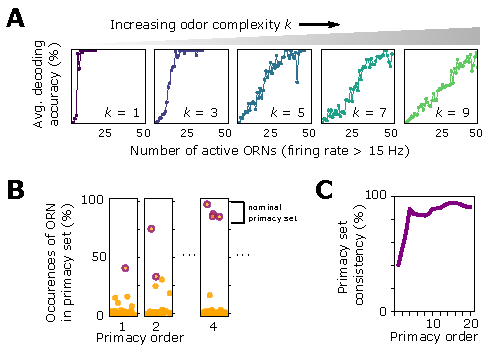
\includegraphics[width=\textwidth]{figures/4_primacy_coding}
		\phantomsubcaption
		\label{fig:primacy_coding_a}	
	\end{subfigure}
	\begin{subfigure}[t]{0\linewidth}
		\phantomsubcaption
		\label{fig:primacy_coding_b}
	\end{subfigure}
	\begin{subfigure}[t]{0\linewidth}
		\phantomsubcaption
		\label{fig:primacy_coding_c}
	\end{subfigure}
	\caption{\footnotesize{
	\textbf{A} Decoding accuracy as a function of the number of active ORNs, for different odor complexities. The primacy set consists of those ORNs required to be active for accurate decoding. %; the set size grows with odor complexity.
	\textbf{B}~Frequency of particular ORNs in primacy sets of an odor placed atop different backgrounds. Individual plots show, for given primacy order $p$, the percentage of backgrounds for which the primacy set of odor A contains a given ORN (dots). Purple dots indicate the $p$ ORNs which most commonly appear in these sets -- i.e. a nominal background-invariant primacy set for odor A. Points are jittered horizontally for visualization.
	\textbf{C}~Consistency of primacy sets across backgrounds, as a function of $p$. Consistency is defined as the likelihood that an ORN in the nomimal primacy set appears in any of the 1000 individual primacy sets, averaged over all ORNs in the nominal set (i.e. average of the y-values of the purple dots in B).
	%\textbf{B} Number of active ORNs required to fully decode odor signals of varying odor intensity and complexity. 
	%\textbf{C} Primacy sets for a step signal in the presence of different background intensities are almost identical for all but the smallest primacy orders  ($p \gtrapprox 5$). Yellow: overlap of the primacy sets for step signal when placed atop a weak (1x) vs. a medium (10x) background; purple: overlap of primacy sets for step signal atop weak vs. strong (100x) backgrounds.
	}}
	\label{fig:primacy_coding}
\end{figure}

Signal transformations in the sensing periphery are propagated through the remainder of the olfactory circuit. How does front-end adaptation interact with these subsequent neural transformations? ORNs expressing the same OR converge to a unique AL glomerulus, where they receive lateral inhibition from other glomeruli~\cite{lateral_inh, lateral_inh_asahina}. This inhibition implements a type of divisive gain control~\cite{divisive_normalization}, normalizing the activity of output projections neurons, which then synapse onto a large number of Kenyon cells (KCs) in the mushroom body. To investigate how odor representations are affected by interactions between front-end ORN adaptation and this lateral inhibition and synaptic divergence, we extended our ORN encoding model by adding uniglomerular connections from ORNs to the antennal lobe, followed by sparse, divergent connections to 2500 KCs~\cite{memory_review, litwinkumar, abbott_axel}. Inhibition was modeled via divisive normalization, with parameters chosen according to experiment~\cite{divisive_normalization}.
We quantified decoding accuracy by training and testing a binary classifier on the KC activity output of sparse odors of distinct intensity and identity, randomly categorized as appetitive or aversive. For simplicity, odor signals of the same identity but differing intensity were assigned the same valence. We trained the classifier on $N_{{\text {ID}}}$ sparse odor identities at intensities chosen randomly over 4 orders of magnitude, then tested the classifier accuracy on the same odor identities but of differing concentrations. 

Classification accuracy degrades to chance level as $N_{\text {ID}}$ becomes very large (Fig.~\ref{fig:downstream_a}). When acting alone, either divisive normalization or ORN adaptation can help, although the effect of ORN adaptation is stronger. When both are active, accuracy improves further, suggesting that these distinct adaptive transformations may act jointly at different stages of neural processing in preserving representations of odor identity. As expected, these gains mostly vanish for the same odors chosen from a narrower range of concentrations (Fig.~S3).

Interestingly, if we train the classifier to distinguish odors by their distinct identity, rather than valence, we find that the benefits conferred by divisive normalization do not appear until $N_{{\text {ID}}}$ is substantial, with accuracy below $65\%$ for $N_{{\text {ID}}} > 50$ (Fig.~\ref{fig:downstream_b}). On the other hand, with ORN adaptation accuracy remains above $85\%$ for more than 1000 odor identities, strongly implicating front-end adaptation as a key player in maintaining odor identity representations, before signals are further processed downstream. 


%{\color{blue} Code with temporal sequence of odors, not strength or subset? Each vector is  the sequence of temporal activation -- does adaptation help? }









%%%%%%%%%%%%%%%%%%%%%%%%%%%%%%%%%%%%%%%%%%%%%%%%%%%%%%%%%%%%%%%%%
%%%%%%%%%%%%	   	        DISCUSSION                %%%%%%%%%%%
%%%%%%%%%%%%%%%%%%%%%%%%%%%%%%%%%%%%%%%%%%%%%%%%%%%%%%%%%%%%%%%%%





\section*{Discussion}

%{\color {blue}-- also don't forget to mention that the odor-receptor  interactions are nonlinear and that saturation is important in this case -- also many odors  Stopfer -- information in each pulse enough (small 50s bins) is enough to classify odors . Go further here and say that even in odor connfounds and complex odors, same conclusion follows. maybe do this for temporal presentation, not odor reconstruction, just order?}

We have found that front-end Weber-Fechner gain control~\cite{srinivas_elife,cafaro_WL,cao_WL},
combined with a short-term adaptation mechanism that depends on the activity of the channels rather than on the identity of the receptor involved~\cite{nagel_wilson_biophysical,martelli,srinivas_elife,si2017invariances}, may contribute significantly to the preservation of neural representations of odor identity in the insect olfactory system, amid confounding odors and intensity fluctuations. Drawing on experimental evidences for a number of ORN-invariant response features, we have emphasized how common adaptative scaling and dynamics across ORNs confer significant benefits in coding fidelity. Nontheless, we have verified that our results hold even when some of these invariances are relaxed. Assuming different adaptation time $\tau_a$ (Fig.~S4) and different adapted activity levels $A_{a0}$ for different ORN types (Fig.~S???), or including possible cooperative effects between multiple binding sites on the same Or-Orco complex (Fig.~S5), does not change our main results.
%These features enhance the coding capacity of ensemble ORN response while helping maintain representations of odor identity independent of intensity (Figs.~\ref{fig:tuning_curves}-\ref{fig:coding}). %It allows robust determination of odor identity from single whiffs when mixed among static backgrounds, and 
%. Increases in the strength and complexity of background odors rapidly scramble odor codes in non-adaptive systems, a degradation that is substantially mitigated with the addition of ORN adaptation.
%When combined with downstream mechanisms, this front-end adaptation mechanism significantly enhances the capacity of the olfactory system to decode odor identity and discriminate new odors from lingering background odors (Figs.~\ref{fig:decoding} and \ref{fig:downstream}). 
%These conclusions are independent of the algorithm used to decode odors, whether it is a compressed sensing scheme that fully reconstruct odor signals from neural response or classification algorithms that categorize odors by identity or valence. 
While our framework incorporates many observed features of the \textit{Drosphila} olfactory system -- Weber-Law adaptation, power-law distributed receptor affinities, temporal filter invariance, connectivity topologies --  it is minimal. We considered only one of the chemoreceptor families expressed in the fly antenna~\cite{chemoreceptors_review} and ignored possible contribution of odor binding proteins~\cite{vogt1981pheromone,menuz2014rna}, inhibitory odorants~\cite{Cao_Tu_WL}, and odorant-odorant antagonism~\cite{reddy2017antagonism}, which could further boost coding capacity and preserve representation sparsity. %We use a simple adaptive nonlinear-linear-nonlinear model that preserves the Weber-Fechner Law and reproduces responses to both naturalistic and Gaussian stimuli~\cite{srinivas_elife}. 
Useful extensions to our simplified nonlinear-linear-nonlinear model might incorporate ephaptic coupling between ORNs housed in the same sensillum~\cite{ephactic}, global inhibition in the mushroom body~\cite{giant_inhibitory_neuron}, and the effects of long-term adaptation~\cite{Guo_Smith}. 

%Possible extensions include %further details such as the complementary kinetics of transduction and spike generation that together preserve response timing independent of intensity~\cite{srinivas_elife}, 
%the ephaptic coupling between neighboring ORNs within the same sensillum~\cite{ephaptic}, which could affect coding capacity by exploiting response bidirectionality, and the effect of long-term (time scales of minutes to hours) adaptation~\cite{Guo_Smith}. 

\begin{figure}[!t]
	\centering
	\begin{subfigure}[t]{\linewidth}
		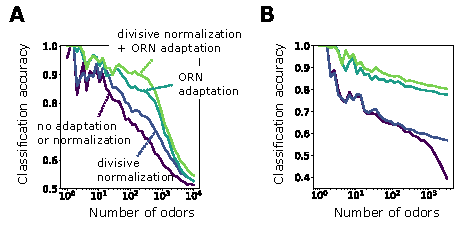
\includegraphics[width=\textwidth]{figures/5_downstream}
		\phantomsubcaption
		\label{fig:downstream_a}	
	\end{subfigure}
	\begin{subfigure}[t]{0\linewidth}
		\phantomsubcaption
		\label{fig:downstream_b}
	\end{subfigure}
	\caption{\footnotesize{
	\textbf{A} Accuracy of binary classification by odor valence, as a function of the number of distinct odor identities classified by the trained network (concentrations span 4 orders of magnitude), in systems with only ORN adaptation, only divisive normalization, both or neither. \textbf{B} Same as (A) but now classifying odors  by identity.
	}}
	\label{fig:downstream}
\end{figure}


Previous studies have characterized various neural mechanisms that help preserve combinatorial codes. 
Lateral inhibition between glomeruli helps tame saturation and boost weak signals~\cite{divisive_normalization}. %ORNs exhibiting both excitatory and inhibitory responses to odorants can increase coding capacity by exploiting response bidirectionality~\cite{Cao_Tu_WL}. In vertebrates, G-protein-coupled chemoreceptors rather than Orco-coupled cation channels, antagonism among odorants may help maintain response sparsity~\cite{reddy2017antagonism}. 
The sparse degree of connectivity to either the olfactory bulb (vertebrates) or mushroom body (in insects) %(in the fly each KC receives connections from only $\sim$7 AL glomeruli) 
may also be precisely tuned to optimize the system's capacity to learn associations~\cite{litwinkumar}. In this work, we find that some of these downstream features act in concert with front-end dynamic adaptation in maintaining representations of odor identity.

Other studies have implicated the unique temporal patterns of neural response as signatures of odor identity~\cite{stopfer_temporal_model, multiple_timescales_stopfer, stopfer_nat_neuro, stopfer_temporal_channel}. ORN and projection neuron time traces form distinct trajectories in low-dimensional projections, and cluster by odor identity, much as we have found here (Fig.~\ref{fig:coding}). In our framework, temporal coding is implicit: because the input nonlinearity depends on the diverse affinities of the receptors for the odorants, %strength of feedback onto Or-Orco activation depends on an ORN's unique response characteristics, 
odor signals are naturally formatted into temporal patterns that are both odor- and ORN-specific --  despite the universality of the adaptation time scale~$\tau$, linear response filter, and rectifier (Figs.~\ref{fig:tuning_curves_d}-\ref{fig:tuning_curves_e}). Further, the fact that decoder memory as short as $\tau_{\textup M} \sim \tau \sim 250$ ms are enough suggest that only brief time windows are needed for accurate odor identification, consistent with previous findings~\cite{stopfer_nat_neuro}. We also find that front-end adaptation enhances the robustness of other combinatorial coding schemes, such as primacy coding~\cite{primacy_coding}, which relies on the temporal order of ORN activation but not absolute firing rate (Fig.~\ref{fig:primacy_coding}).

In the well-characterized chemosensory system of bacterial chemotaxis, Weber Law adaptation is enacted through a feedback loop from the output activity of the receptor-kinase complexes onto the enzymes modifying the receptors sensitivity~\cite{EmonetReview}. It is interesting that some aspects of this architecture are also present in ORNs: although the molecular players are different (and still largely unknown), it has been shown that transduction activity feeds back onto Or-Orco cation channel opening, enabling the Weber-Fechner relation~\cite{nagel_wilson_biophysical,srinivas_elife,cao_WL}. 
That this adaptation mechanism appears to act similarly across ORNs~\cite{srinivas_elife,martelli,cao_WL} suggests the involvement of the universal co-receptor Orco, whose role in long-term adaptation has recently been demonstrated~\cite{getahun2013insect,getahun2016intracellular,Guo_Smith}.  

In sensory systems, Weber Law adaptation ensures that systems remain in the regime of maximum sensitivity, broadening dynamic range and maintaining information capacity~\cite{adaptation_fairhall}.
%, laughlin, deweese_adaptation}. 
%Doing so requires matching sensory response to attributes of the environment, either by adapting to specific stimuli or to stimuli statistics~\cite{adaptation_fairhall}. 
For a single-channel system, this requires matching the midpoint of the dose-response curve to the mean ligand concentration~\cite{information_theory_adaptation}, a strategy which may fail in multi-channel systems with overlapping tuning curves: adaptation to one signal could inhibit identification of others, if the signals excite some but not all of the same sensors. 
Our results show that this strategy is still largely functional. This can be traced to the observation that in CS, accuracy is guaranteed when sufficiently distinct odor identities produce sufficiently distinct ORN responses, a condition known as the restricted isometry property~\cite{CS_tao}. Indeed, the Weber-Fechner scaling increases the likelihood that this property  is satisfied, beyond that in the non-adaptive system (SI text and Figs.~S6-S7). Still, restricted isometry does not require that response repertoires are \textit{invariant} to environmental changes. That is, even if the subset of active ORNs were concentration-dependent, odors could still in principle be fully reconstructible by CS.
Nonetheless, our results in t-SNE clustering (Fig.~\ref{fig:coding}), primacy coding  (Fig.~\ref{fig:primacy_coding_b}-\ref{fig:primacy_coding_c}), and odor classification (Fig.~\ref{fig:downstream}) suggest that such response invariance is a natural byproduct of front-end adaptation. Together, this implies that Weber Law adaptation, whether required by the olfactory circuit for precise signal reconstruction (as in CS) or for developing odor associations (as in classification), can play an integral part in maintaining combinatorial codes amid changing environmental conditions.

%Viewing sensory systems as input/output machines, the role of adaptation is therefore to maintain information capacity in dynamic environments~\cite{information_theory_adaptation}. 
%For a single-channel, information capacity is increased by matching the midpoint of the nonlinear dose-response curve, where sensitivity is highest, to mean ligand concentration according to Weber-Fechner law~\cite{information_theory_adaptation}. 

%universal adaption: adaptation to one odor could adversely affect identification of a new odor, if the latter excites some but not all of the same ORNs. In compressed sensing, signal reconstruction requires that odor signals produce sufficiently distinct responses, a mathematical condition known as the restricted isometry property. Our results show that front-end adaptation  preserves this property, helping maintain combinatorial representations of odor identity despite the broad overlaps in the tuning curves of the receptors.



%%%%%%%%%%%%%%%%%%%%%%%%%%%%%%%%%%%%%%%%%%%%%%%%%%%%%%%%%%%%%%%%%
%%%%%%%%%%%%	   	           METHODS                %%%%%%%%%%%
%%%%%%%%%%%%%%%%%%%%%%%%%%%%%%%%%%%%%%%%%%%%%%%%%%%%%%%%%%%%%%%%%




\section*{Methods}
%\subsection*{Mathematical model}
Equations~\ref{eq:steady_state_act_OR}-\ref{eq:adaptation_dynamics} are integrated numerically using the Euler method with a 2 ms time step. %The odor-binding and Or/Orco activation dynamics are assumed competitive (complexes bind at most one odorant), described for each complex $a$ by a 2(N`+1)-state system $\{C_a, C^*_a,  C_a\text{-}s_i, C^*_a\text{-}s_i\}$ with kinetics $C_a \rightleftharpoons s_i\text{-}C_a$, $C^*_a \rightleftharpoons s_i\text{-}C^*_a$, $C_a \rightleftharpoons C^*_a$, and $C_a\text{-}s_i \rightleftharpoons C^*_a\text{-}s_i$. 
%The first two of these describe the odor binding dynamics, with equilibrium constants $K_{ai}$ and $K^*_{ai}$, respectively. The latter two describe activation, with rate constants $w_{a,\pm} \propto (1 + \exp(\pm \epsilon_a))$ and $w_{a,\pm}^* \propto (1 + \exp(\pm \epsilon_{a,i}))$, respectively. 
%Assuming detailed balance produces Eq.~\ref{eq:steady_state_act_OR} for the steady state active fraction of complexes of class $a$ (SI). 
For ORN firing (Eq.~\ref{eq:firing_machinery}), $h(t)$ is bi-lobed~\cite{martelli}: $h(t) = Ap_{\textup{Gam}}(t; \alpha_1, \tau_1) - Bp_{\textup{Gam}}(t; \alpha_2, \tau_2)$, $A = 190$, $B = 1.33$,  $\alpha_1=2$, $\alpha_2=3$, $\tau_1 = 0.012$, and $\tau_2 = 0.016$, where $p_{\textup{Gam}}$ is the pdf of Gamma($\alpha$, $1/\tau$). Nonlinearity $f$ is modeled as a linear rectifier with 5 Hz threshold.
For t-SNE dimensionality reduction, ORN responses were generated for odor signal combinations consisting of 1 (among 10) distinct foreground odors A atop 1 (among 50) distinct background odors B, each of complexity $K = 5$, for Fig.~\ref{fig:coding_a}.  Fig.~\ref{fig:coding_b} plots responses for 10 odors ($K = 5$) at 40 concentrations spanning 4 decades, atop a random sparse background odor ($K = 5)$ of similar magnitude.
%Mutual information was calculated from 1000 randomly chosen sparse odor identities ($K = 4$ for both odor A and odor B), with noise $\sigma \sim \mathcal{N}(0, \textup{1e-3})$ added to $A_a$. 

For compressed sensing decoding, sparse components $s_i$ are chosen as $s_i = s_0 + \Delta s_i$ where $s_0$ is set as the center of linearization and $\Delta s_i \sim \mathcal {N} (s_0/3, s_0/9)$. Reconstructed signal components $\hat {s} _i = s_0 + \Delta s_i$ are computed by minimizing $\sum_i |\Delta s_i|$ subject to $\Delta r_a = \sum_i dr_a/ds_i\big|_{s_0}\Delta  s_i$ where $\Delta r_a = r_a(\mathbf s) -  r_a(s_0)$ are the ``excess” ORN firing rates about the linearization point. For static stimuli, $\epsilon_a$ equals the fixed point of Eq.~\ref{eq:adaptation_dynamics} in response to the background stimulus. For fluctuating stimuli, $\epsilon_a$ is updated in time by continuously integrating  $r_a(t)$, via Eqs.~\ref{eq:adaptation_dynamics} and~\ref{eq:firing_machinery}; thus, only knowledge of $r_a(t)$ is needed by the decoder.
The naturalistic odor signal (Fig.~\ref{fig:decoding_d}) was generated by randomly varying flow rates of ethyl acetate and measuring the concentration with a photo-ionization detector~\cite{srinivas_elife}. Statistics mirroring a turbulent flow~\cite{celani} were verified (Fig.~S8).

For the network model, the AL-to-MB connectivity matrix $\mathbf {J}_1$, is chosen such that  each KC connects pre-synaptically to 7 randomly chosen AL glomeruli~\cite{litwinkumar,abbott_axel}. The results shown in Fig.~\ref{fig:downstream} are an average of 10 distinct instantiations of this random topology. The $Z=2500$ KCs are then connected by a matrix $\mathbf J_2$ to a readout layer of dimension $Q$, where $Q=2$ for binary and $Q=N_{\text{ID}}$ for multi-class classification. Both AL-to-MB and MB-to-readout connections are perceptron-type with rectified-linear thresholds. The weights of $\mathbf J_1$ and $\mathbf J_2$ are chosen randomly from $\sim \mathcal{N}(0, 1/\sqrt{7})$ and $\sim \mathcal{N}(0, 1/\sqrt{Z})$, respectively. Only the $\mathbf J_2$ and the MB-to-output thresholds are updated during supervised network training, via logistic regression (for binary classification) or its higher-dimensional generalization, the softmax cross entropy (for multi-class classification).


\bibliography{bibliography}

\acknow{NK was supported by the Swartz Foundation. We thank DA Clark, JR Carlson, M Demir, S Gorur-Shandilya, H Mattingly, and ???? for comments on the manuscript.}
\showacknow


\end{document}